\documentclass[12pt]{article}

\usepackage[utf8]{inputenc}
\usepackage{graphicx}
\usepackage[portuguese]{babel}
\usepackage{float}

\title{MAC0344 Arquitetura de Computadores\\
Lista de Exercícios No. 2
}
\author{Mateus Agostinho dos Anjos\\NUSP 9298191}
\date{\today}

\begin{document}
	\maketitle
	\begin{itemize}
		\item[1 -]
			\hfill\\
			\begin{itemize}
				\item[a)]
					\hfill \\
					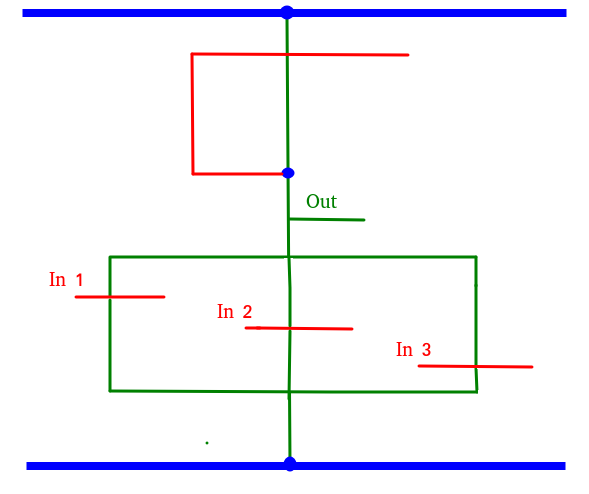
\includegraphics[width=5cm]{porta_NOR_3_entradas.png}
				\item[b)]
					\hfill \\
					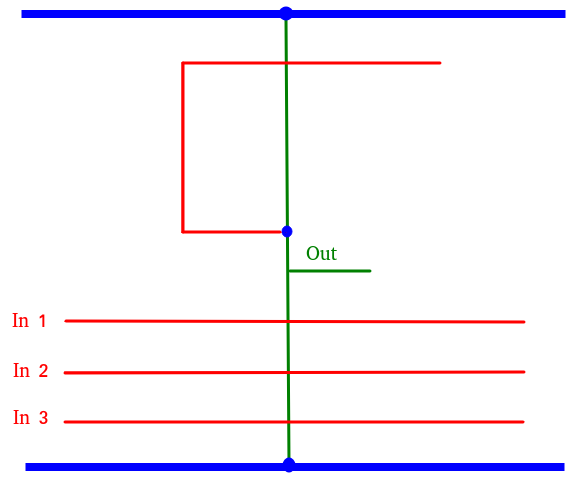
\includegraphics[width=5cm]{porta_NAND_3_entradas.png}
			\end{itemize}
		\item[2 -]
			Quando conduzindo eletricidade, o transistor MOS apresenta
			resistência efetiva de condução $r_{ef} = \alpha L/W$,
			portanto alternativa \textbf{(b)}.
		\item[3 -]
			A tecnologia do momento é \textbf{CMOS}, portanto
			alternativa \textbf{(b)}.
	\end{itemize}
\end{document}